\documentclass[a4paper, 11pt]{article}
\usepackage[utf8]{inputenc} % Change according your file encoding
\usepackage{graphicx}
\usepackage{url}

%opening
\title{Seminar Report: Opty}
\author{Maria Gabriela Valdes and Victoria Beleuta}
\date{\today{}}

\begin{document}

\maketitle

\section{Introduction}

During this lab, we implemented a transaction server using optimistic concurrency control in Erlang . Opty is a concurrency control method applied to transactional systems such as relational database management systems. It assumes that multiple transactions can complete without interfering with each other, while using data resources without acquiring locks. Before committing, each transaction checks if any other transaction has changed the entry. If it hasn't been changed the transation can commit, if there are conflicts, the transaction rollsback and restarts.
 
\section{Work done}

We have completed the code files provided to correctly implement the algorithm. Our source code can be found in the src folder. To start the algorithm locally you have to call the function \textit{start} of module \textit{opty} with six arguments in the following order: number of clients, number of entries, number of updates, number of reads, duration of experiments and size of the subset of entries to be used by each client. For example: opty:start(3,4,1,1,5,2). With this command the Opty algorithm will start with three clients, and a store with four entries, one write operation, one read operation, with a duration of 5 seconds and a subset of 2 entries out of the total provided. \\\\
To start the algorithm with the server and clients in different Erlang nodes you first have to start two different Erlang environments. For example:
\begin{itemize}
\item In one terminal type erl -sname optyserver. This will represent an Erlang node name optyserver@server.\\
\item In another different terminal type erl -sname clients. This will represent a Erlang node name clients@server.\\
\end{itemize}
%
First we start the server in the node optyserver@server with the command \textit{opty:start\_server(10)}, where 10 is the number of entries. To start the clients you have to call, in the clients node, the function \textit{start\_clients} of module \textit{opty} with seven arguments: number of clients, number of entries, number of updates, number of reads, duration of experiments, the name of the server’s node and the size of the subset of entries. For example: 
\textit{opty:start\_clients(5, 10, 1, 1, 5, optyserver@server, 3)}.\\

\section{Experiments}

\textbf{In the same machine:}\\\\
\textbf{i)} different number of concurrent clients in the system;\\
We ran the following commands to see how the algorithm runs:\\
\begin{itemize}
\item opty:start(1,10,1,1,5,3)\\
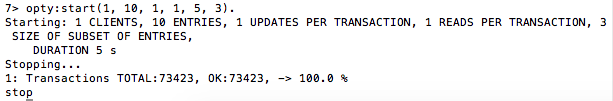
\includegraphics[scale=0.5]{images/exp-i-1.png} \\
\item opty:start(5,10,1,1,5,3)\\
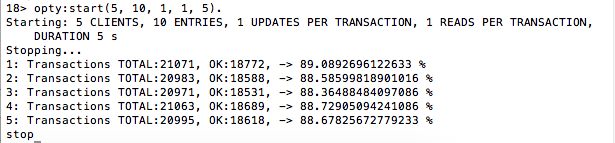
\includegraphics[scale=0.5]{images/exp-i-2.png} \\
\item opty:start(10,10,1,1,5,3)\\
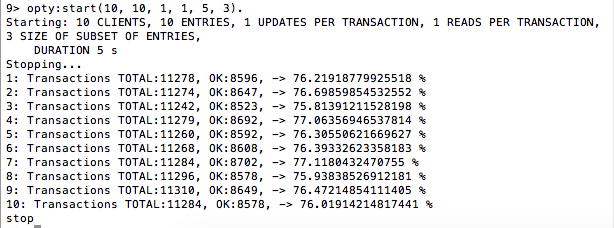
\includegraphics[scale=0.5]{images/exp-i-3.png} \\
\item opty:start(20,10,1,1,5,3)\\
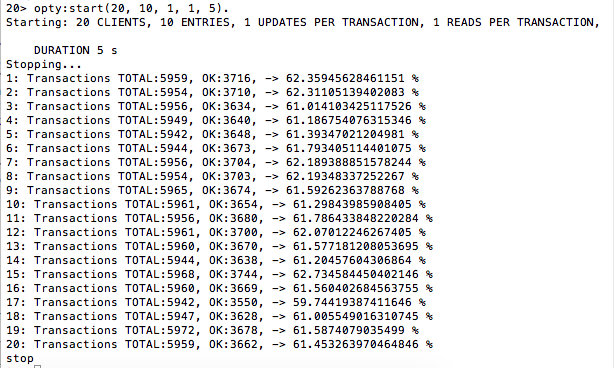
\includegraphics[scale=0.5]{images/exp-i-4.png} \\
\item opty:start(40,10,1,1,5,3)\\
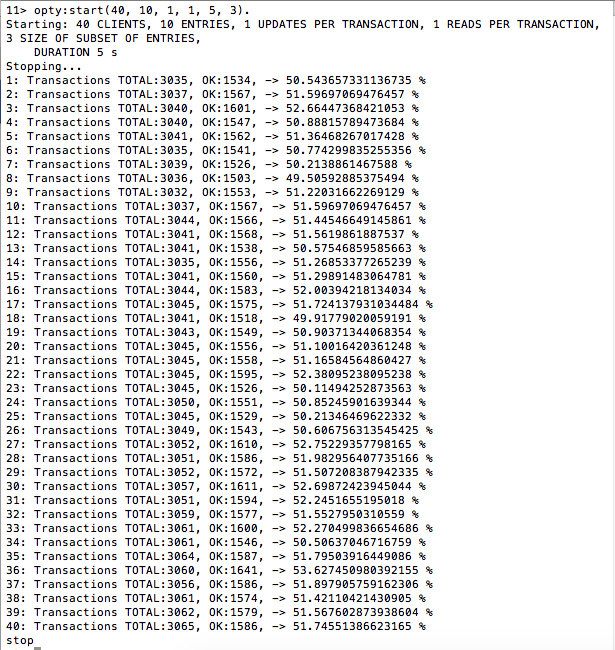
\includegraphics[scale=0.5]{images/exp-i-5.png} \\
\item opty:start(80,10,1,1,5,3)\\
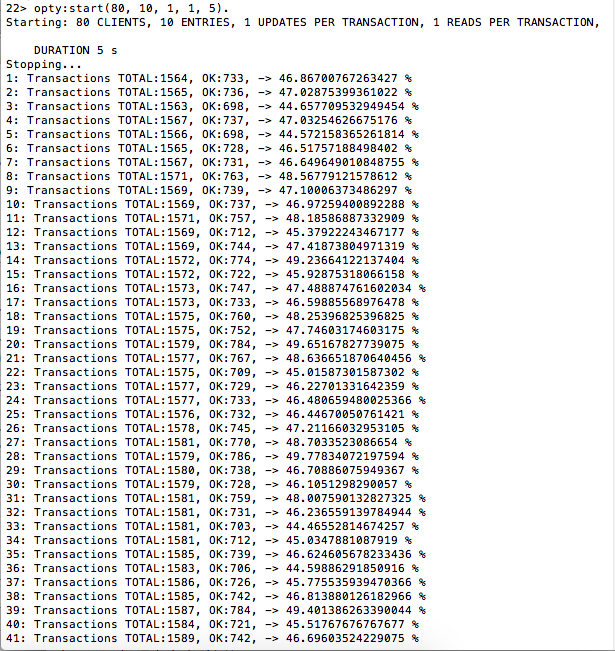
\includegraphics[scale=0.4]{images/exp-i-6a.png} \\
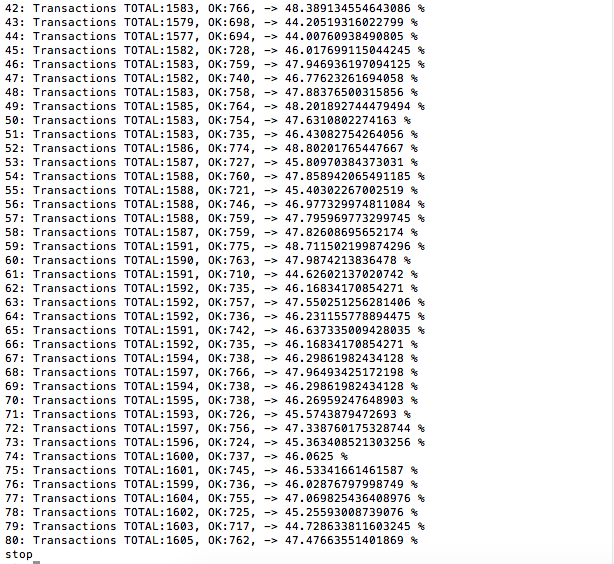
\includegraphics[scale=0.4]{images/exp-i-6b.png} \\
\end{itemize}
%
\newpage
\textbf{ii)} different number of entries in the store;\\
We ran the following commands to see how the algorithm runs:\\
\begin{itemize}
\item opty:start(5,1,1,1,1,1)\\
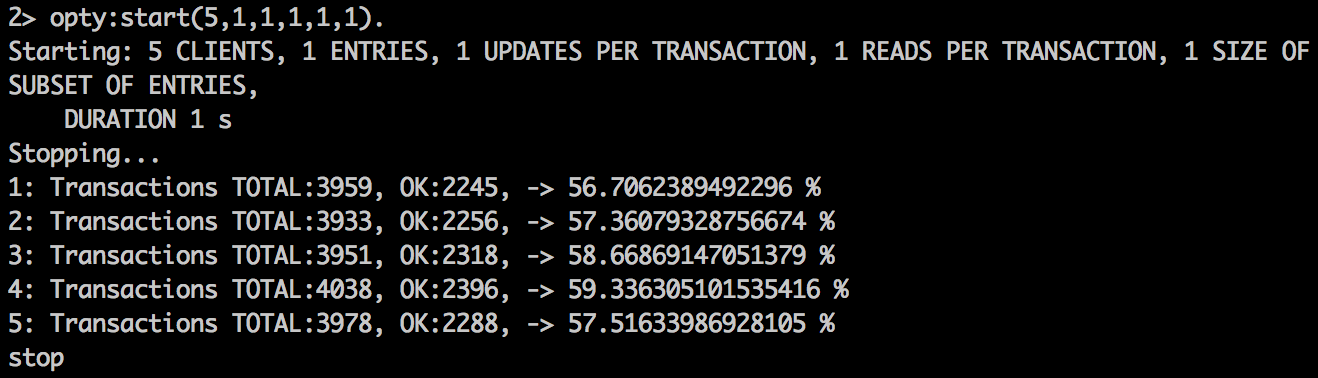
\includegraphics[scale=0.5]{images/exp-ii-1.png} \\
\item opty:start(5,3,1,1,1,3)\\
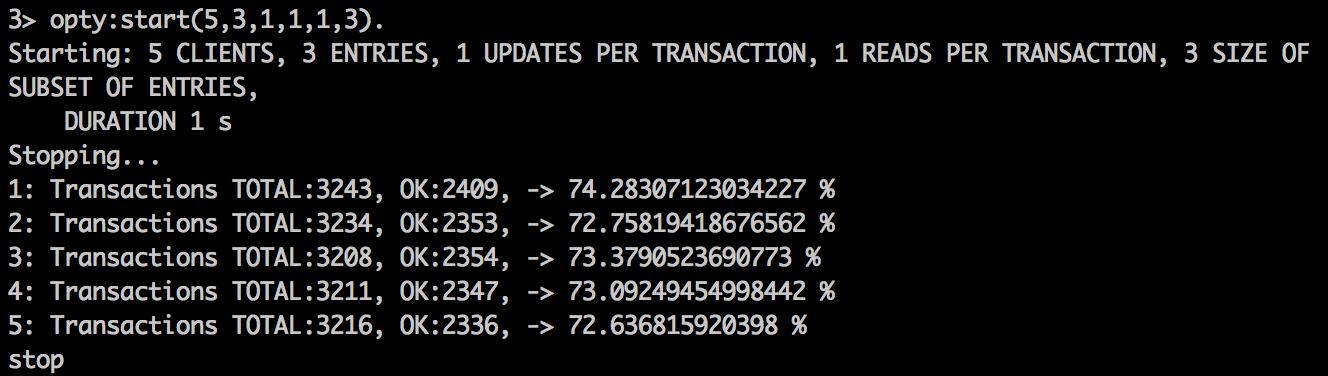
\includegraphics[scale=0.5]{images/exp-ii-2.png} \\
\item opty:start(5,5,1,1,1,5)\\
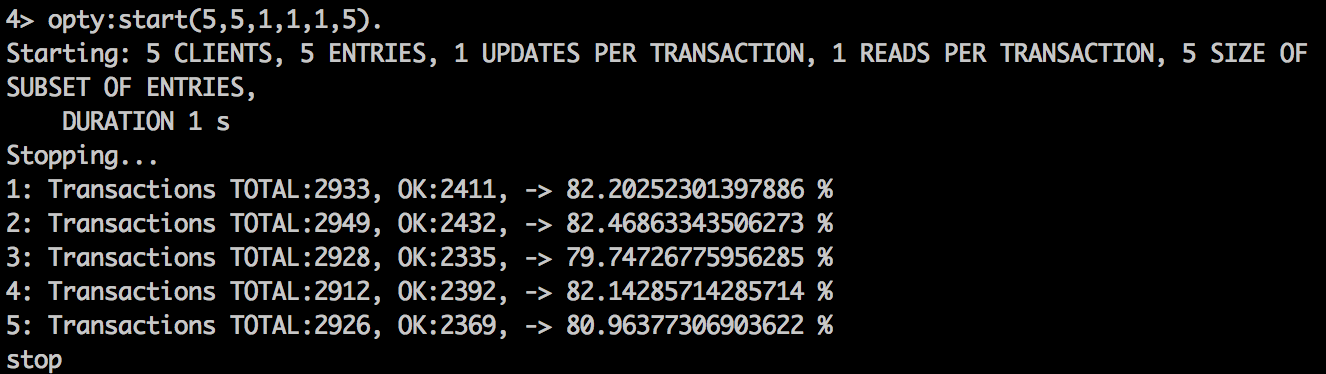
\includegraphics[scale=0.5]{images/exp-ii-3.png} \\
\item opty:start(5,10,1,1,1,10)\\
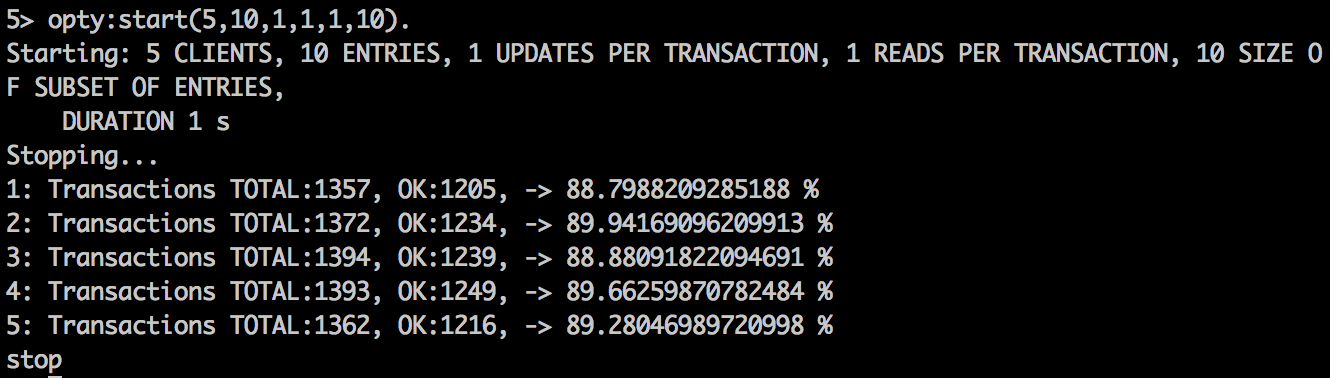
\includegraphics[scale=0.5]{images/exp-ii-4.png} \\
\item opty:start(5,100,1,1,1,100)\\
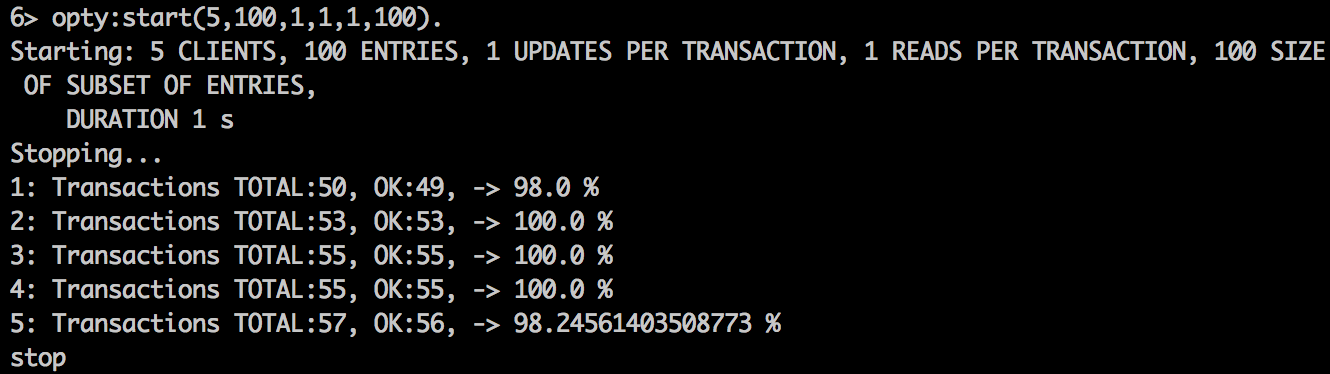
\includegraphics[scale=0.5]{images/exp-ii-5.png} \\
\item opty:start(5,1000,1,1,1,1000)\\
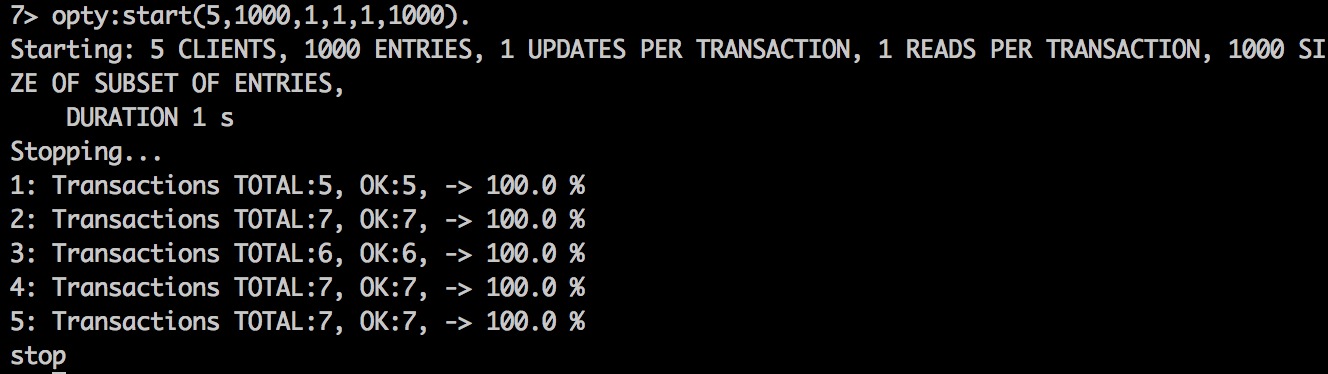
\includegraphics[scale=0.5]{images/exp-ii-6.png} \\
\end{itemize}
%
\textbf{iii)} different number of write operations per transaction;\\
We ran the following commands to see how the algorithm runs:\\
\begin{itemize}
\item opty:start(5,10,1,1,5,3)\\
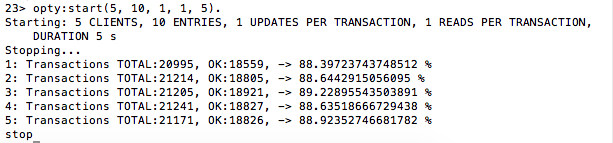
\includegraphics[scale=0.5]{images/exp-iii-1.png} \\
\item opty:start(5,10,5,1,5,3)\\
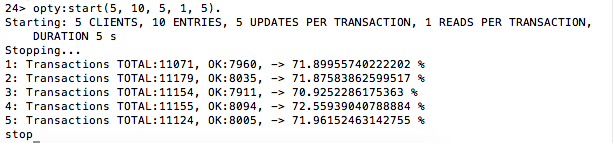
\includegraphics[scale=0.5]{images/exp-iii-2.png} \\
\newpage
\item opty:start(5,10,10,1,5,3)\\
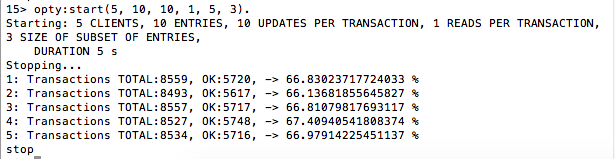
\includegraphics[scale=0.5]{images/exp-iii-3.png} \\
\item opty:start(5,10,20,1,5,3)\\
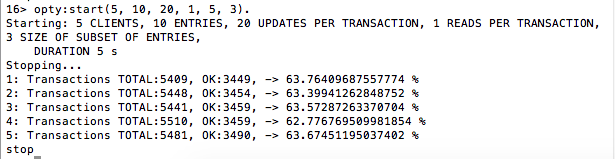
\includegraphics[scale=0.5]{images/exp-iii-4.png} \\
\item opty:start(5,10,40,1,5,3)\\
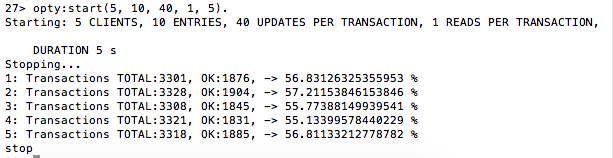
\includegraphics[scale=0.5]{images/exp-iii-5.png} \\
\item opty:start(5,10,80,1,5,3)\\
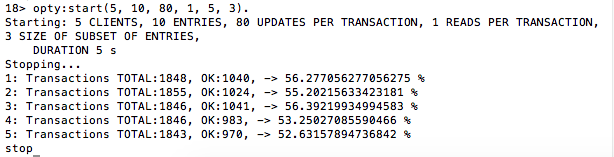
\includegraphics[scale=0.5]{images/exp-iii-6.png} \\
\end{itemize}
%
\newpage
\textbf{iv)} different ratio of read and write operations per transaction;\\
We ran the following commands to see how the algorithm runs:\\
\begin{itemize}
\item opty:start(5,10,2,4,1,5)\\
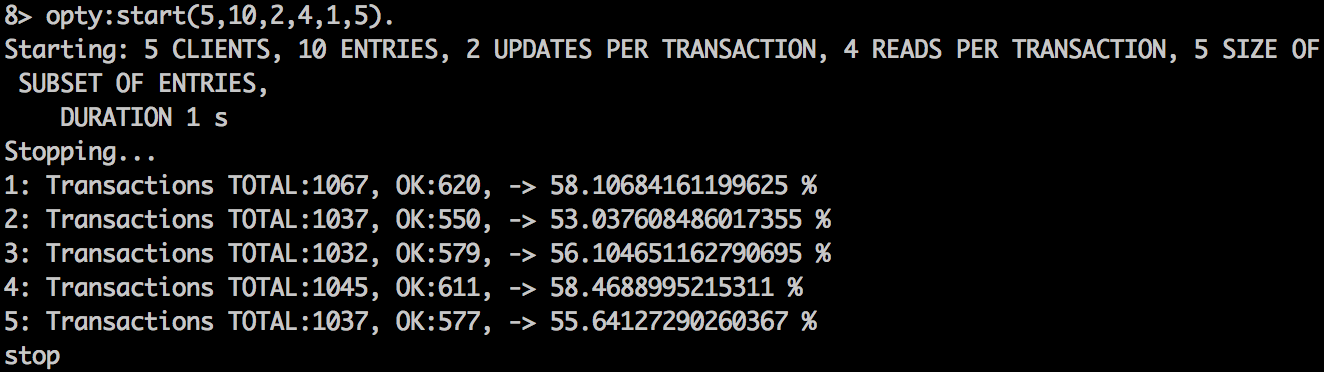
\includegraphics[scale=0.5]{images/exp-iv-1.png} \\
\item opty:start(5,10,4,2,1,5)\\
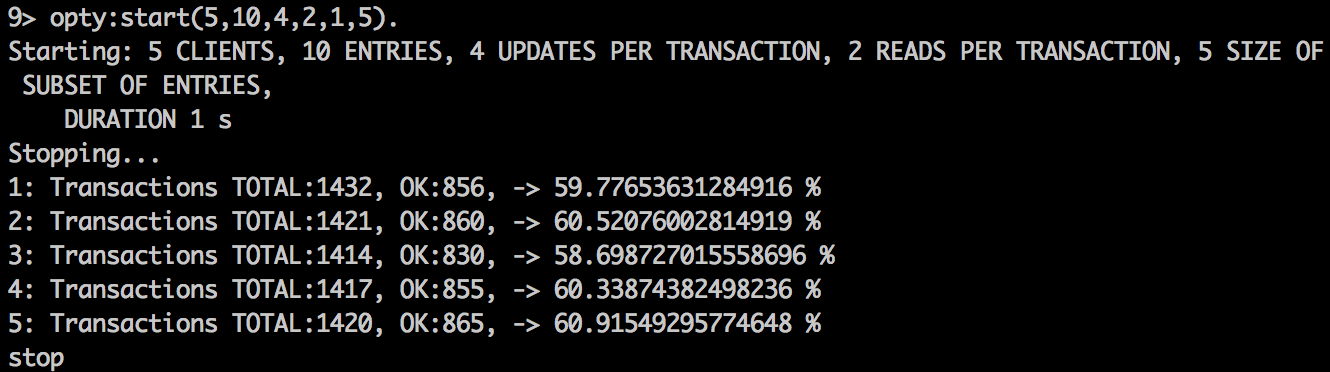
\includegraphics[scale=0.5]{images/exp-iv-2.png} \\
\item opty:start(5,10,3,9,1,5)\\
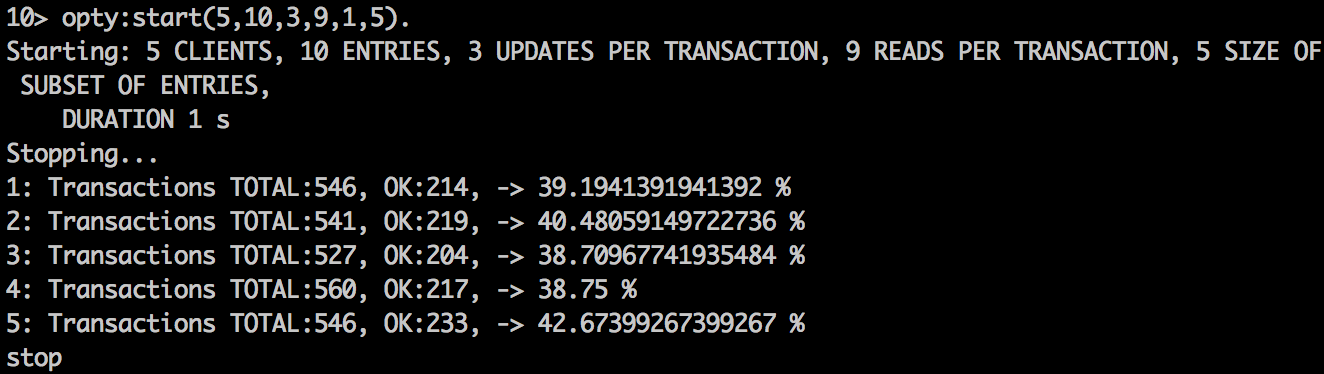
\includegraphics[scale=0.5]{images/exp-iv-3.png} \\
\item opty:start(5,10,9,3,1,5)\\
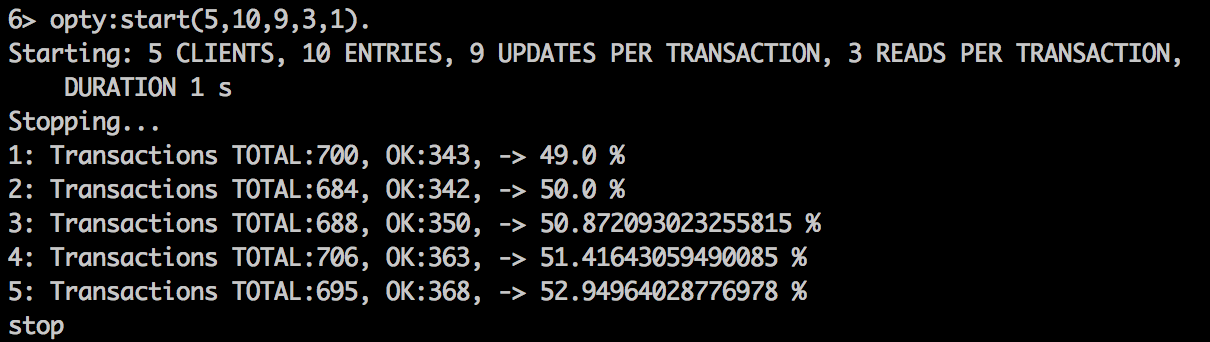
\includegraphics[scale=0.5]{images/exp-iv-4.png} \\
\newpage
\item opty:start(5,10,1,10,1,5)\\
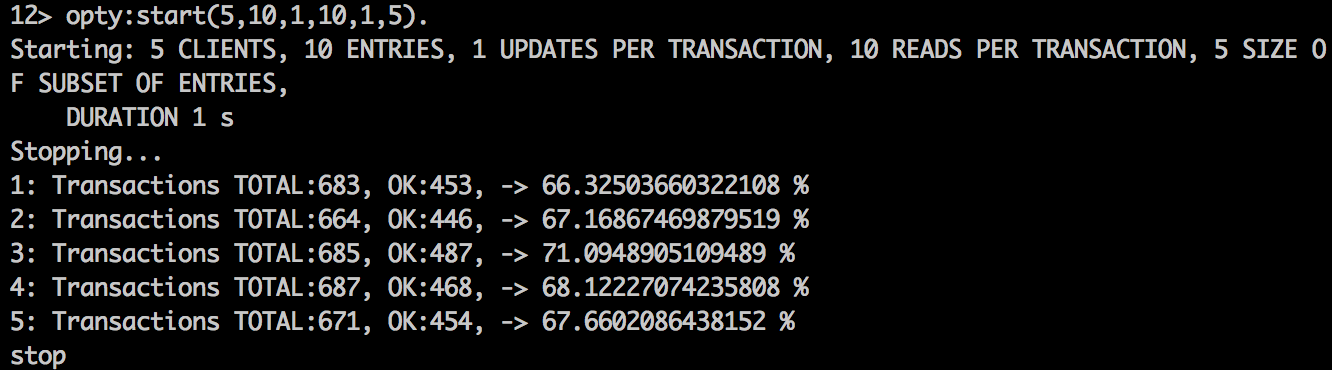
\includegraphics[scale=0.5]{images/exp-iv-5.png} \\
\item opty:start(5,10,10,1,1,5)\\
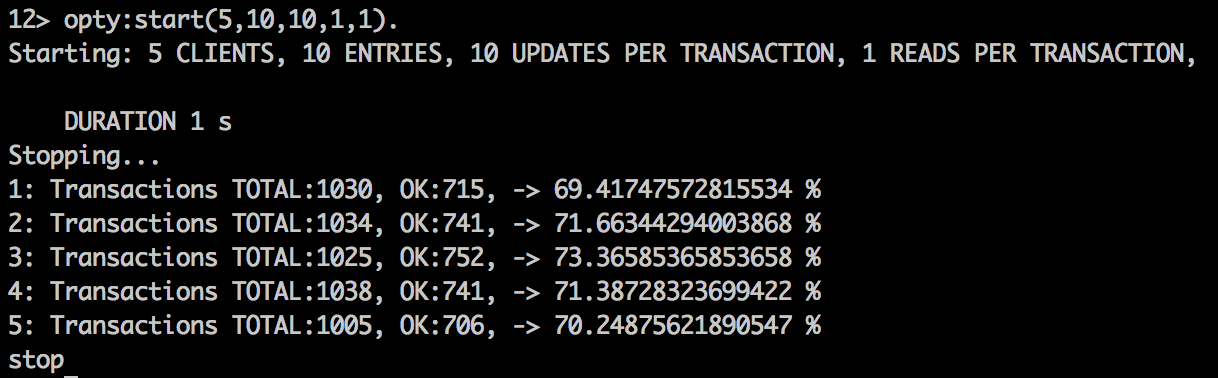
\includegraphics[scale=0.5]{images/exp-iv-6.png} \\
\item opty:start(5,10,1,100,1,5)\\
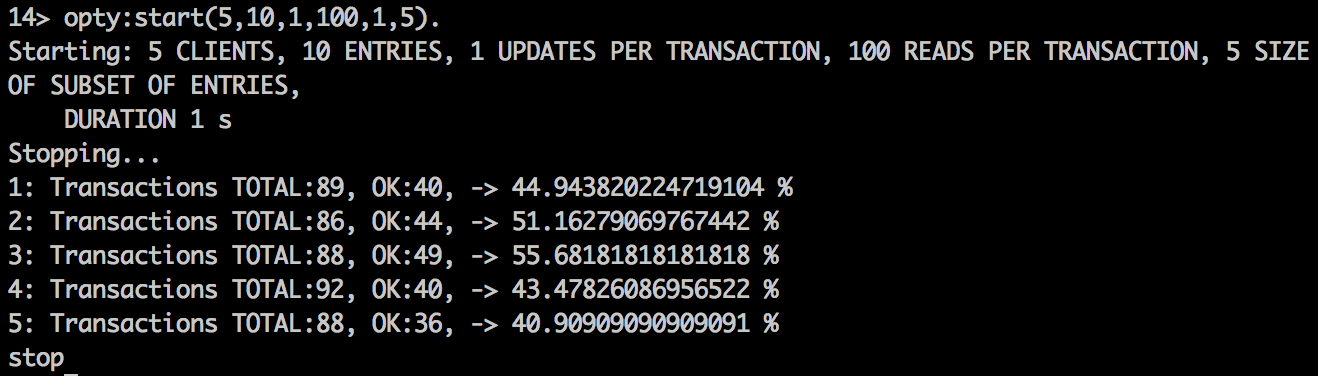
\includegraphics[scale=0.5]{images/exp-iv-7.png} \\
\item opty:start(5,10,100,1,1,5)\\
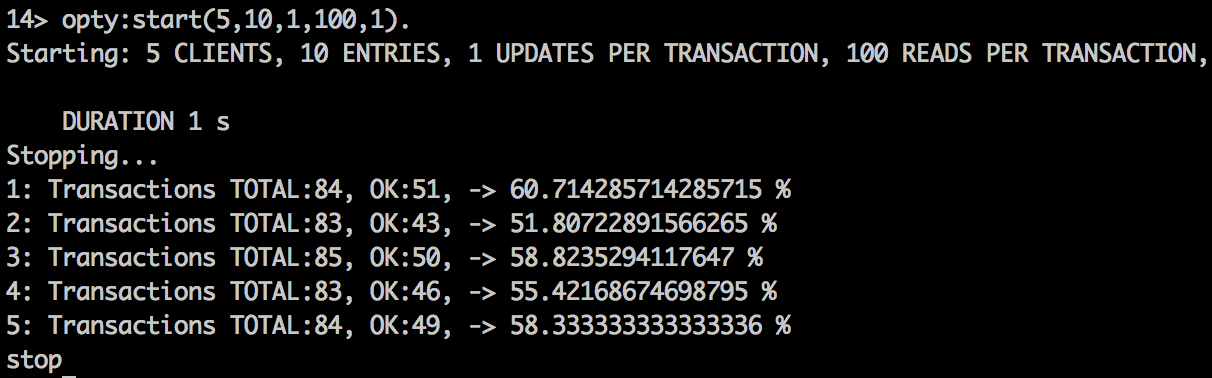
\includegraphics[scale=0.5]{images/exp-iv-8.png} \\
\end{itemize}
%
\newpage
\textbf{v)} different percentage of accessed entries with respect to the total number of entries;\\
We ran the following commands to see how the algorithm runs:\\
\begin{itemize}
\item opty:start(5,10,2,2,1,2)\\
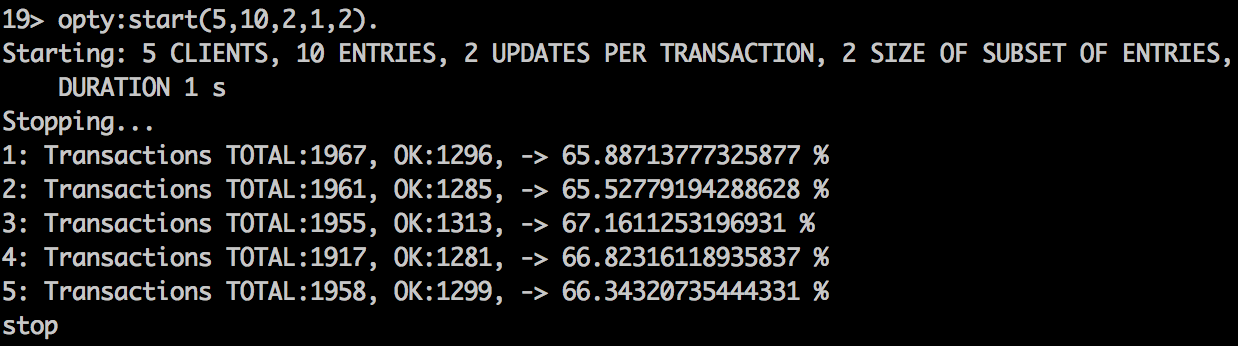
\includegraphics[scale=0.5]{images/exp-v-1.png} \\
\item opty:start(5,10,2,2,1,3)\\
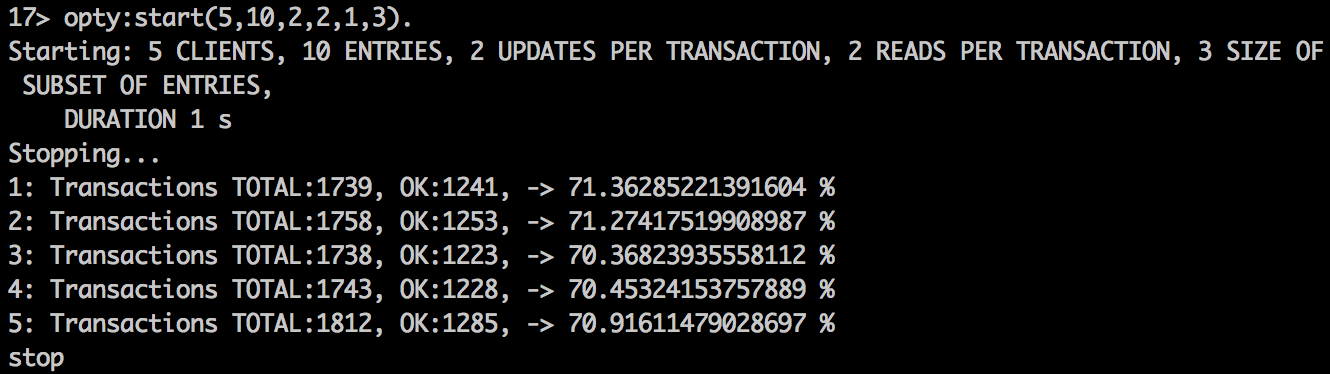
\includegraphics[scale=0.5]{images/exp-v-2.png} \\
\item opty:start(5,10,2,2,1,4)\\
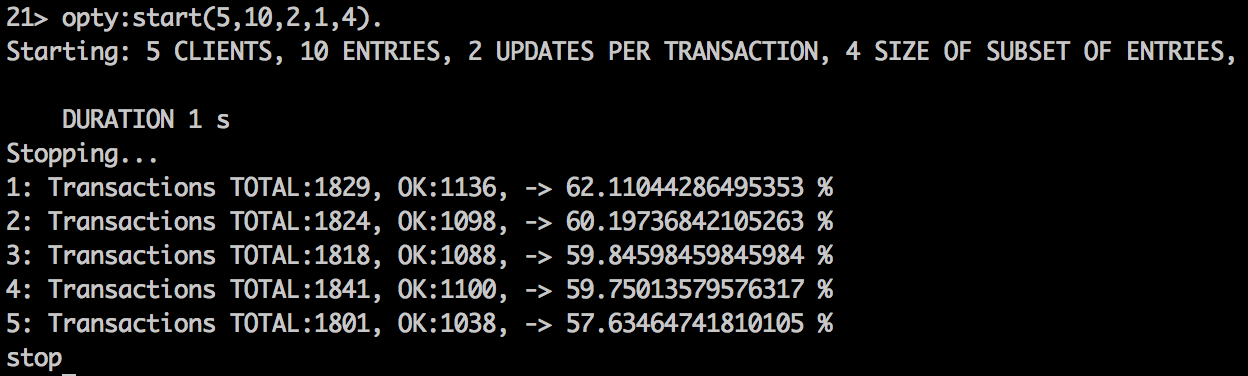
\includegraphics[scale=0.5]{images/exp-v-3.png} \\
\item opty:start(5,10,2,2,1,5)\\
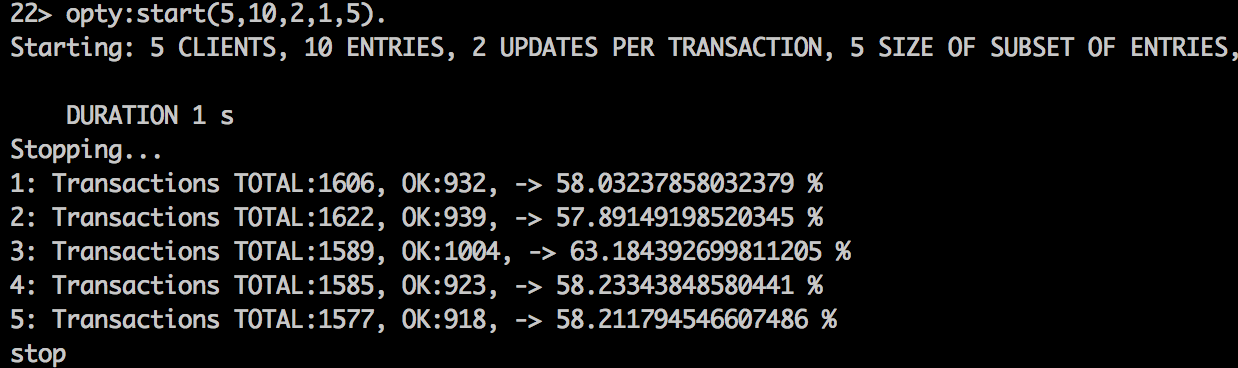
\includegraphics[scale=0.5]{images/exp-v-4.png} \\
\item opty:start(5,10,2,2,1,8)\\
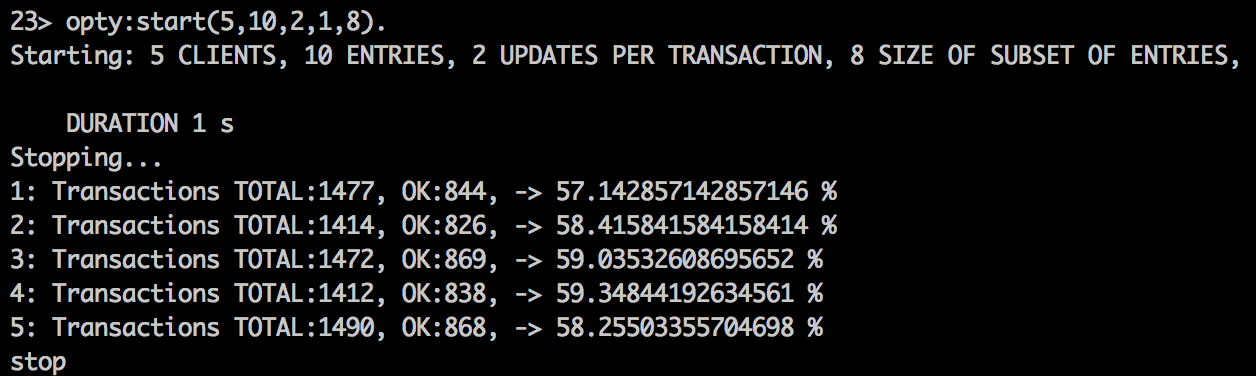
\includegraphics[scale=0.5]{images/exp-v-5.png} \\
\end{itemize}

\textbf{In different machines:}\\\\

We created the server node: optyserver@localhost and ran the command \textit{opty:start\_server(10)}. Then we created the clients node: clients@localhost and ran the command \textit{opty:start\_clients(5, 10, 1, 1, 5, optyserver@server, 3)}.\\\\
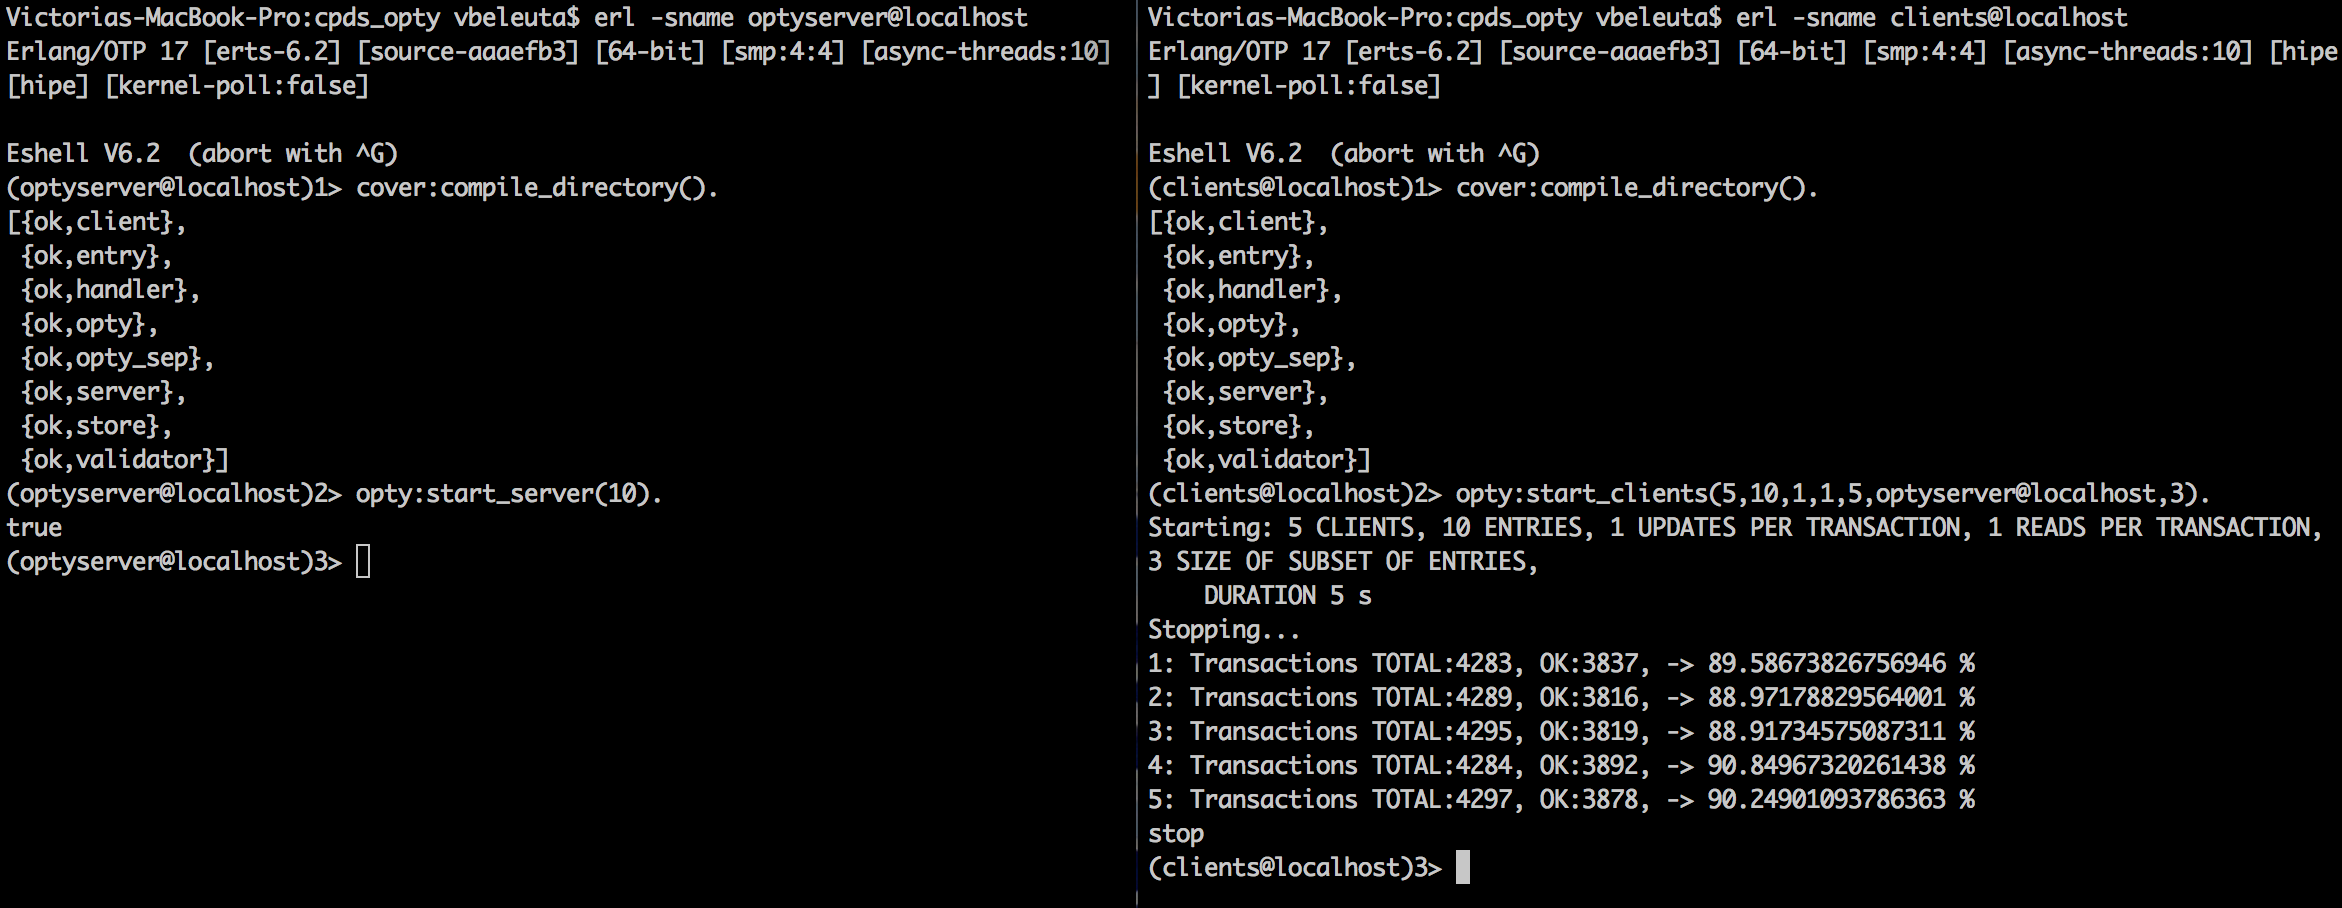
\includegraphics[scale=0.39]{images/distributed.png} \\\\

\newpage
\section{Open questions}

\textbf{1)} What is the impact of each of these parameters on the success rate? Is the success rate the same for the different clients?\\

The success rate is influenced by all of these paramenters:\\
\begin{itemize}
\item For the experiment \textit{i} we see that as we increase the number of clients, the success rate decreases.\\
\item For the experiment \textit{ii} however, we see that as we increase the number of entries, the success rate also increases, because there are less possibilities of conflicts arrising with write operations when we have a larger pool of entries to chose from.\\
\item For experiment \textit{iii} as expected the more write operations we try to perform the more conflicts arrise forcing transactions to restart and their success rate decreases.\\
\item For experiment \textit{iv} the different ratio of reads and writes doesnt influence as much the success rate as in previous cases.\\
\item For experiment \textit{v} the success rate is higher if we choose a smaller subset of our entries.\\
\end{itemize}
In all experiments though the success rate between clients stays almost equal and balanced.\\\\
%
\textbf{2)} If we run this in a distributed Erlang network, where is the handler running?\\
In a distributed network the handler runs in the clients node such that when the clients are destroyed so is the handler.\\\\

\section{Personal opinion}
During this seminar we got an indepth view of how the Optimistic Concurrency Control algorithm works both locally and in a distributed environment. In our opinion, this lab had the right level of difficulty for this course and the amount of time available to us. \\

\end{document}
